\section{Grundlagen}

\begin{frame}[t]\frametitle{Gliederung: Grundlagen}
\tableofcontents[
currentsection,
subsectionstyle=show/show/hide
]
\end{frame}

\subsection{Kristallgitter}
\label{grnd:gitter}
\begin{frame}[c]\frametitle{Kristallgitter}
	Das Kristallgitter in Metallen:
	\begin{itemize}
		\item{Kubisch-primitives Gitter (simple cubic)}
		\item{Kubisch-raumzentriertes Gitter (body centered cubic)}
		\item{Kubisch-flächenzentriertes Gitter (face centered cubic)}
	\end{itemize}
\end{frame}

\begin{frame}[c]
	\centering
	Kubisch-raumzentriertes Gitter
	\\
	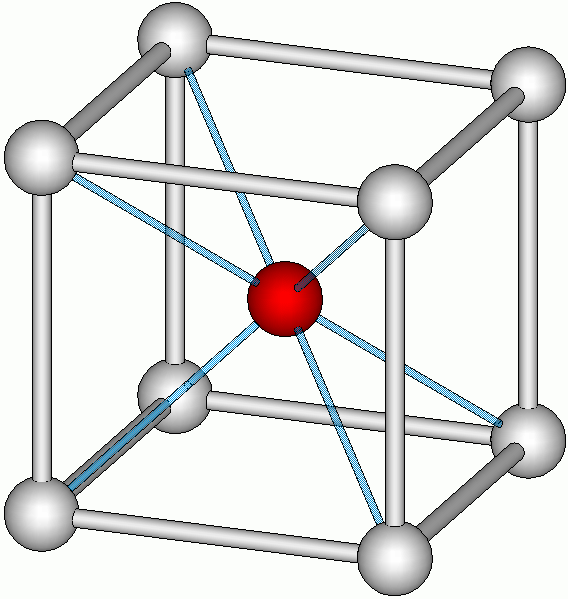
\includegraphics[height=0.4\textwidth]{medien/Krz.png}
	\\
	\tiny{ alpha-/ delta-Fe; beta-Ti, beta-Zr, Cr, V, Mg, Mo, W, Ta, Li, Na, K}
	\\
	\tiny{Quelle:https://de.wikibooks.org/wiki/Werkstoffkunde\_Metall/\_Innerer\_Aufbau/\_Struktur}
\end{frame}

\begin{frame}[c]
	\centering
	Kubisch-flächenzentriertes Gitter
	\\
	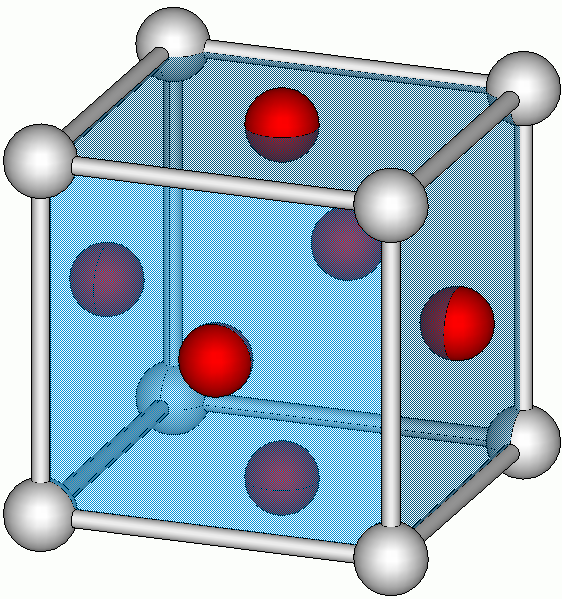
\includegraphics[height=0.4\textwidth]{medien/Kfz.png}
	\\
	\tiny{ gamma-Fe, beta-Co, Cu, Pt, Al, Au, Ag, Pb}
	\\
	\tiny{Quelle:https://de.wikibooks.org/wiki/Werkstoffkunde\_Metall/\_Innerer\_Aufbau/\_Struktur}
\end{frame}

\subsection{Legierungen}
\label{grnd:legierungen}
\begin{frame}[c]\frametitle{Legierung}
	Bronze (Metall-Metall Legierung).
	\begin{itemize}
		\item{Erste von Menschen genutzte Legierung.}
		\item{Kupfer und Zinn (CuSn)}
		\item{Härter als reines Kupfer}
		\item{ca 3300v. Chr. in Palästina}
	\end{itemize}
\end{frame}

\begin{frame}[c]\frametitle{Legierung}
	Eisen
	\begin{itemize}
		\item{Wichtigste binäre Legierung Kohlenstoff}
		\item{Stahl bis 2,06\% Kohlenstoff}
		\item{Gusseisen bis 6,67\% Kohlenstoff}
	\end{itemize}
\end{frame}

\begin{frame}[c]\frametitle{Eisen-Kohlenstoff-Diagramm}
	\centering
	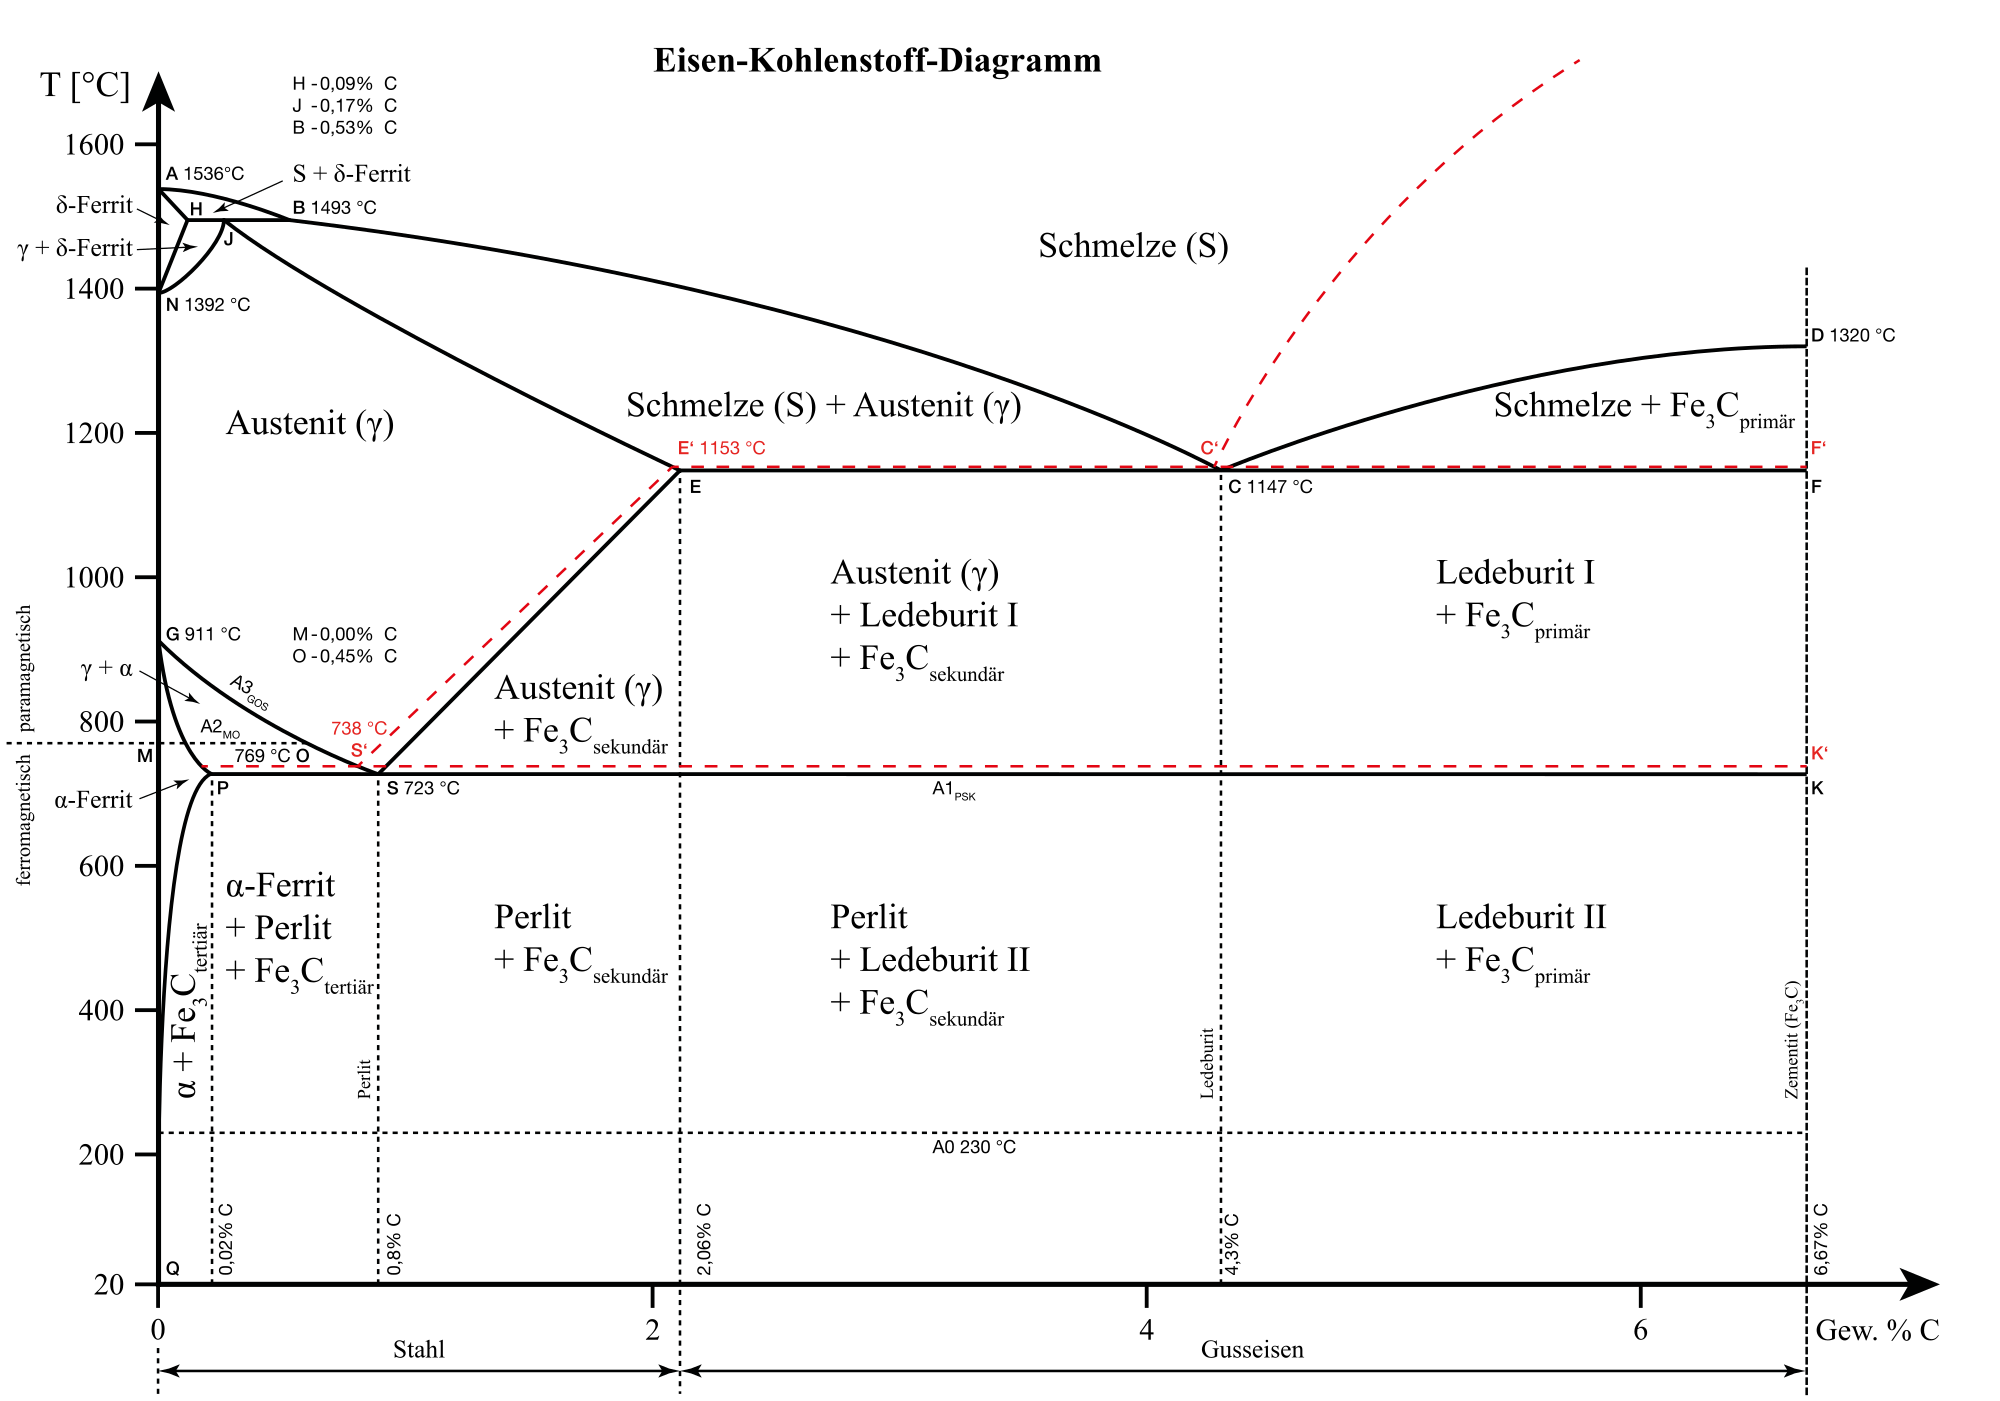
\includegraphics[height=0.5\textwidth]{medien/ekd.png}
	\\
	\tiny{Quelle:https://de.wikipedia.org/wiki/Eisen-Kohlenstoff-Diagramm}
\end{frame}

\subsection{Spannung und Dehnung}
\begin{frame}[c]\frametitle{Spannung und Dehnung}
	\centering
	Spannungs-Dehnungs-Diagramm mit ausgeprägter Streckgrenze
	\\
	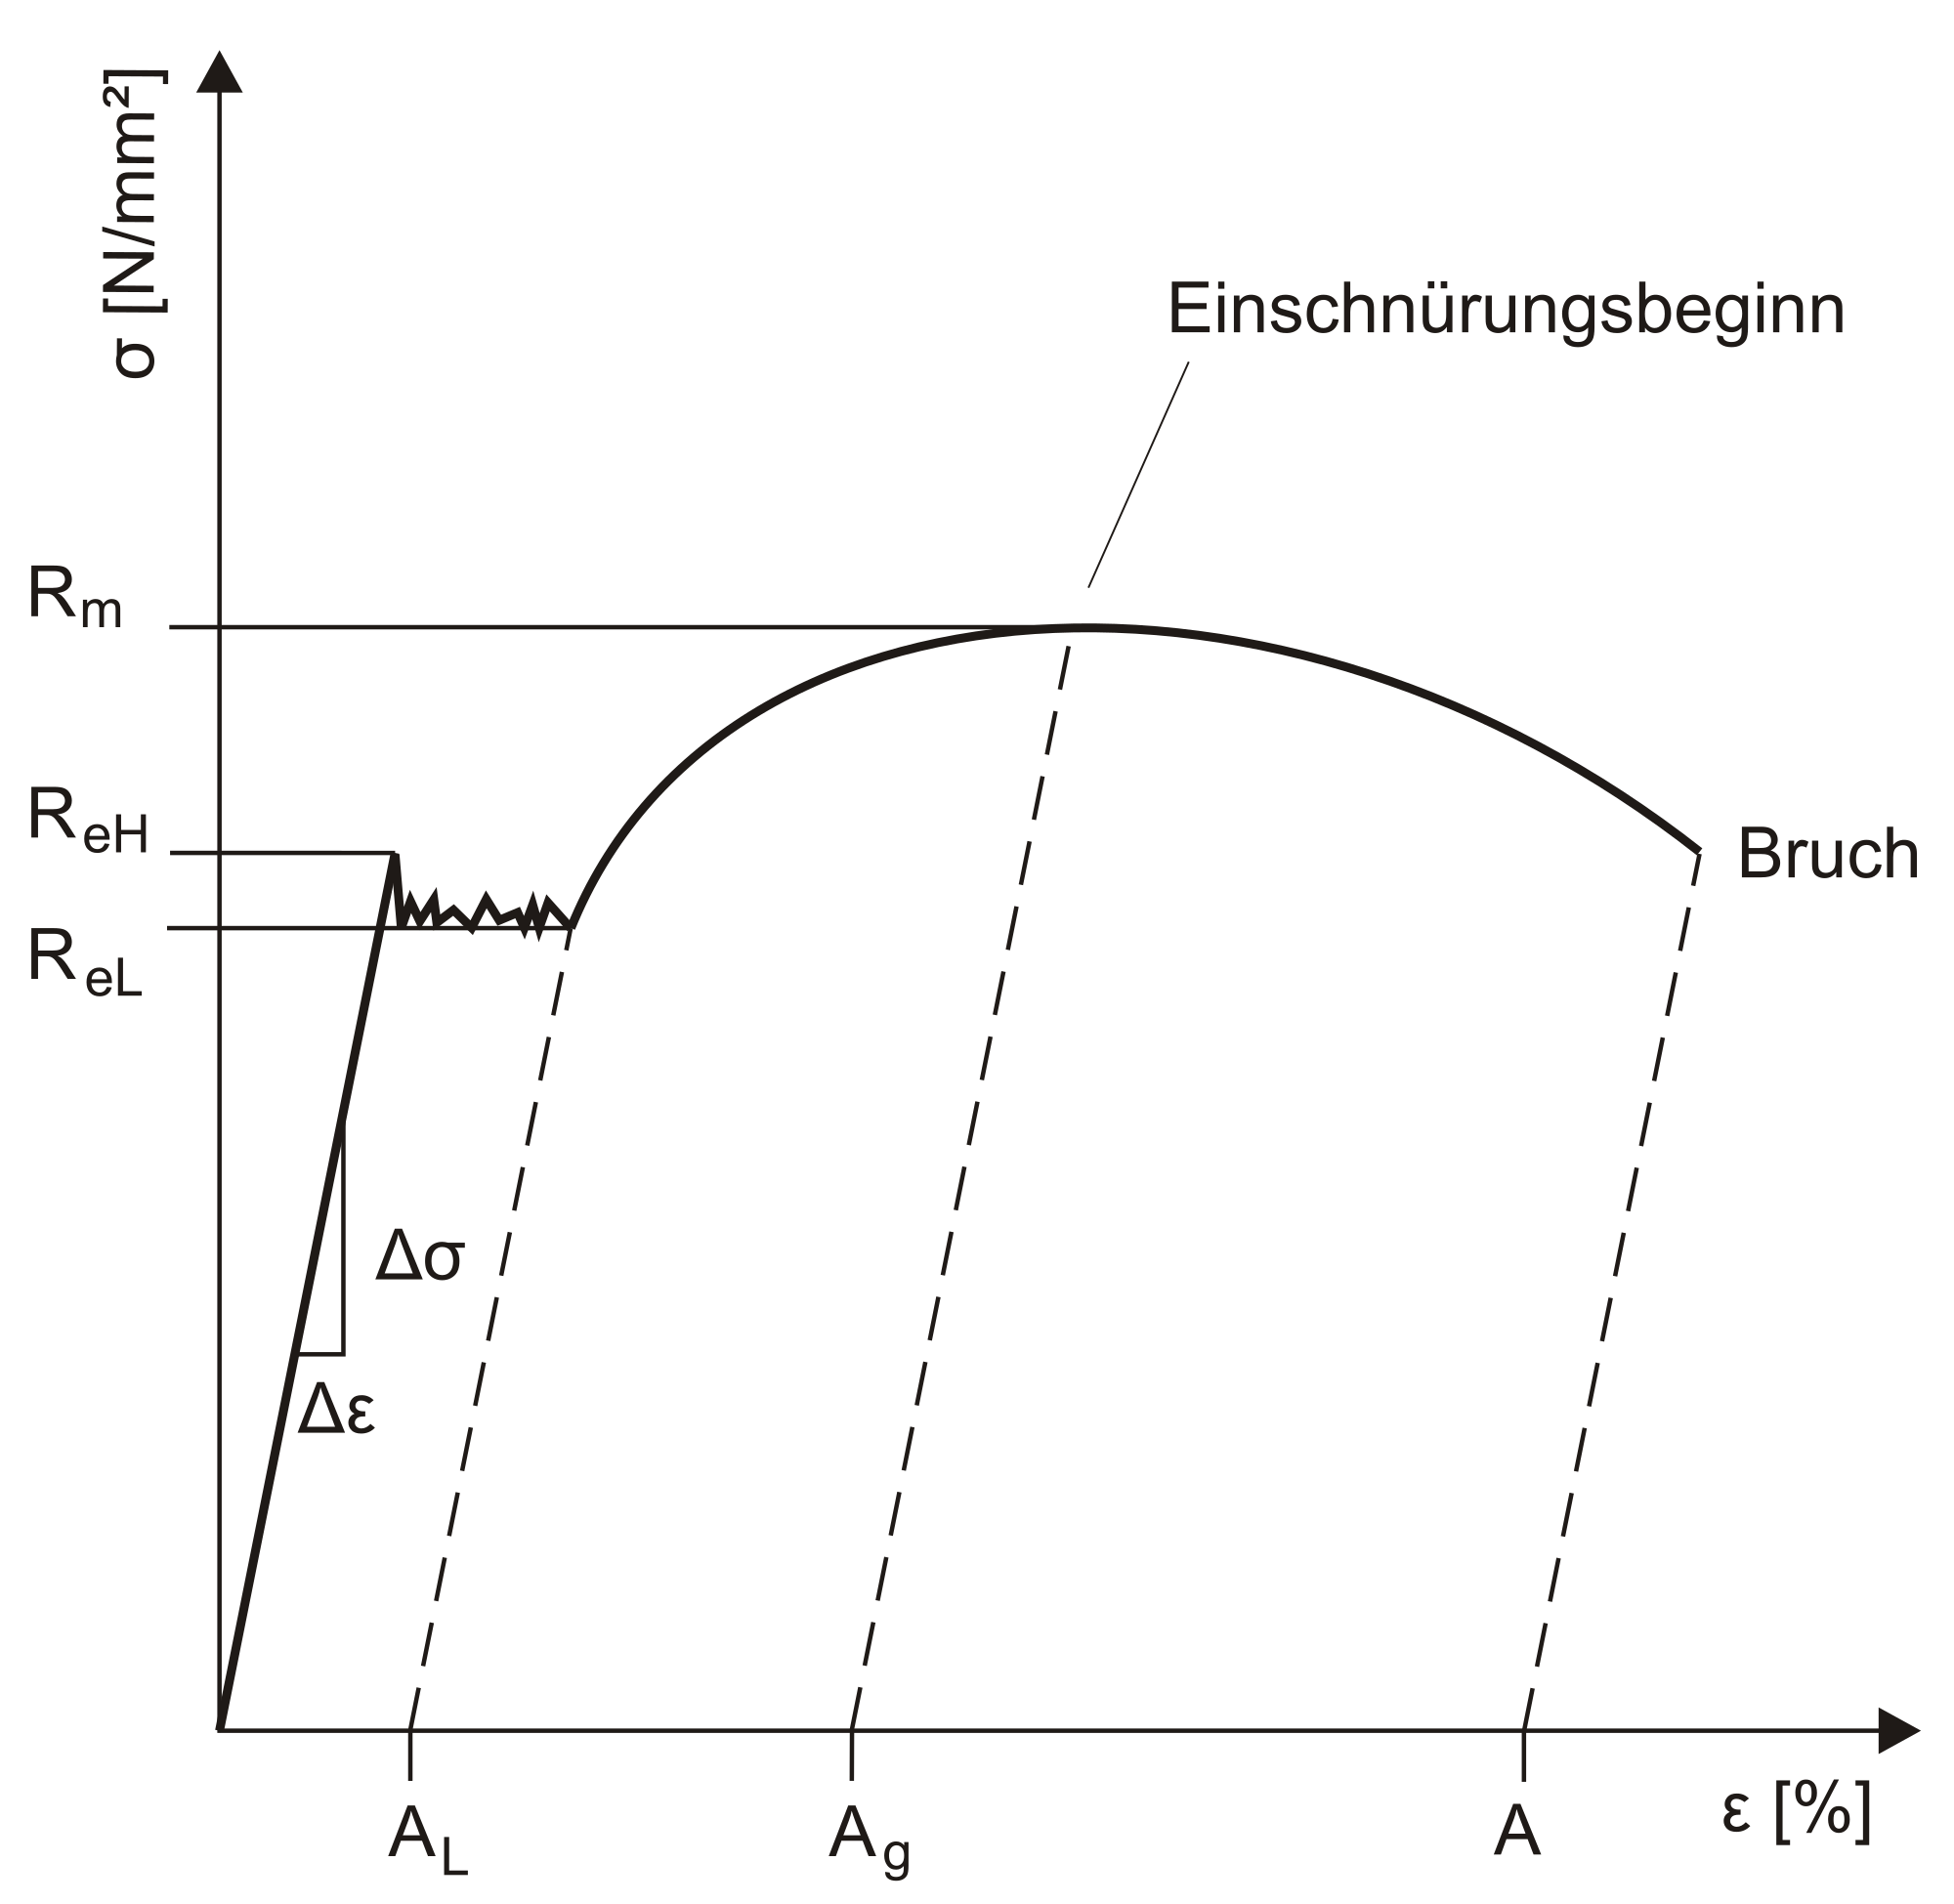
\includegraphics[height=0.5\textwidth]{medien/Spgs-Dehnungs-Kurve_Streckgrenze.png}
	\\
	\tiny{Quelle:https://de.wikipedia.org/wiki/Spannungs-Dehnungs-Diagramm}
\end{frame}

\begin{frame}[c]\frametitle{Spannung und Dehnung}
	\centering
	Spannungs-Dehnungs-Diagramm
	\\
	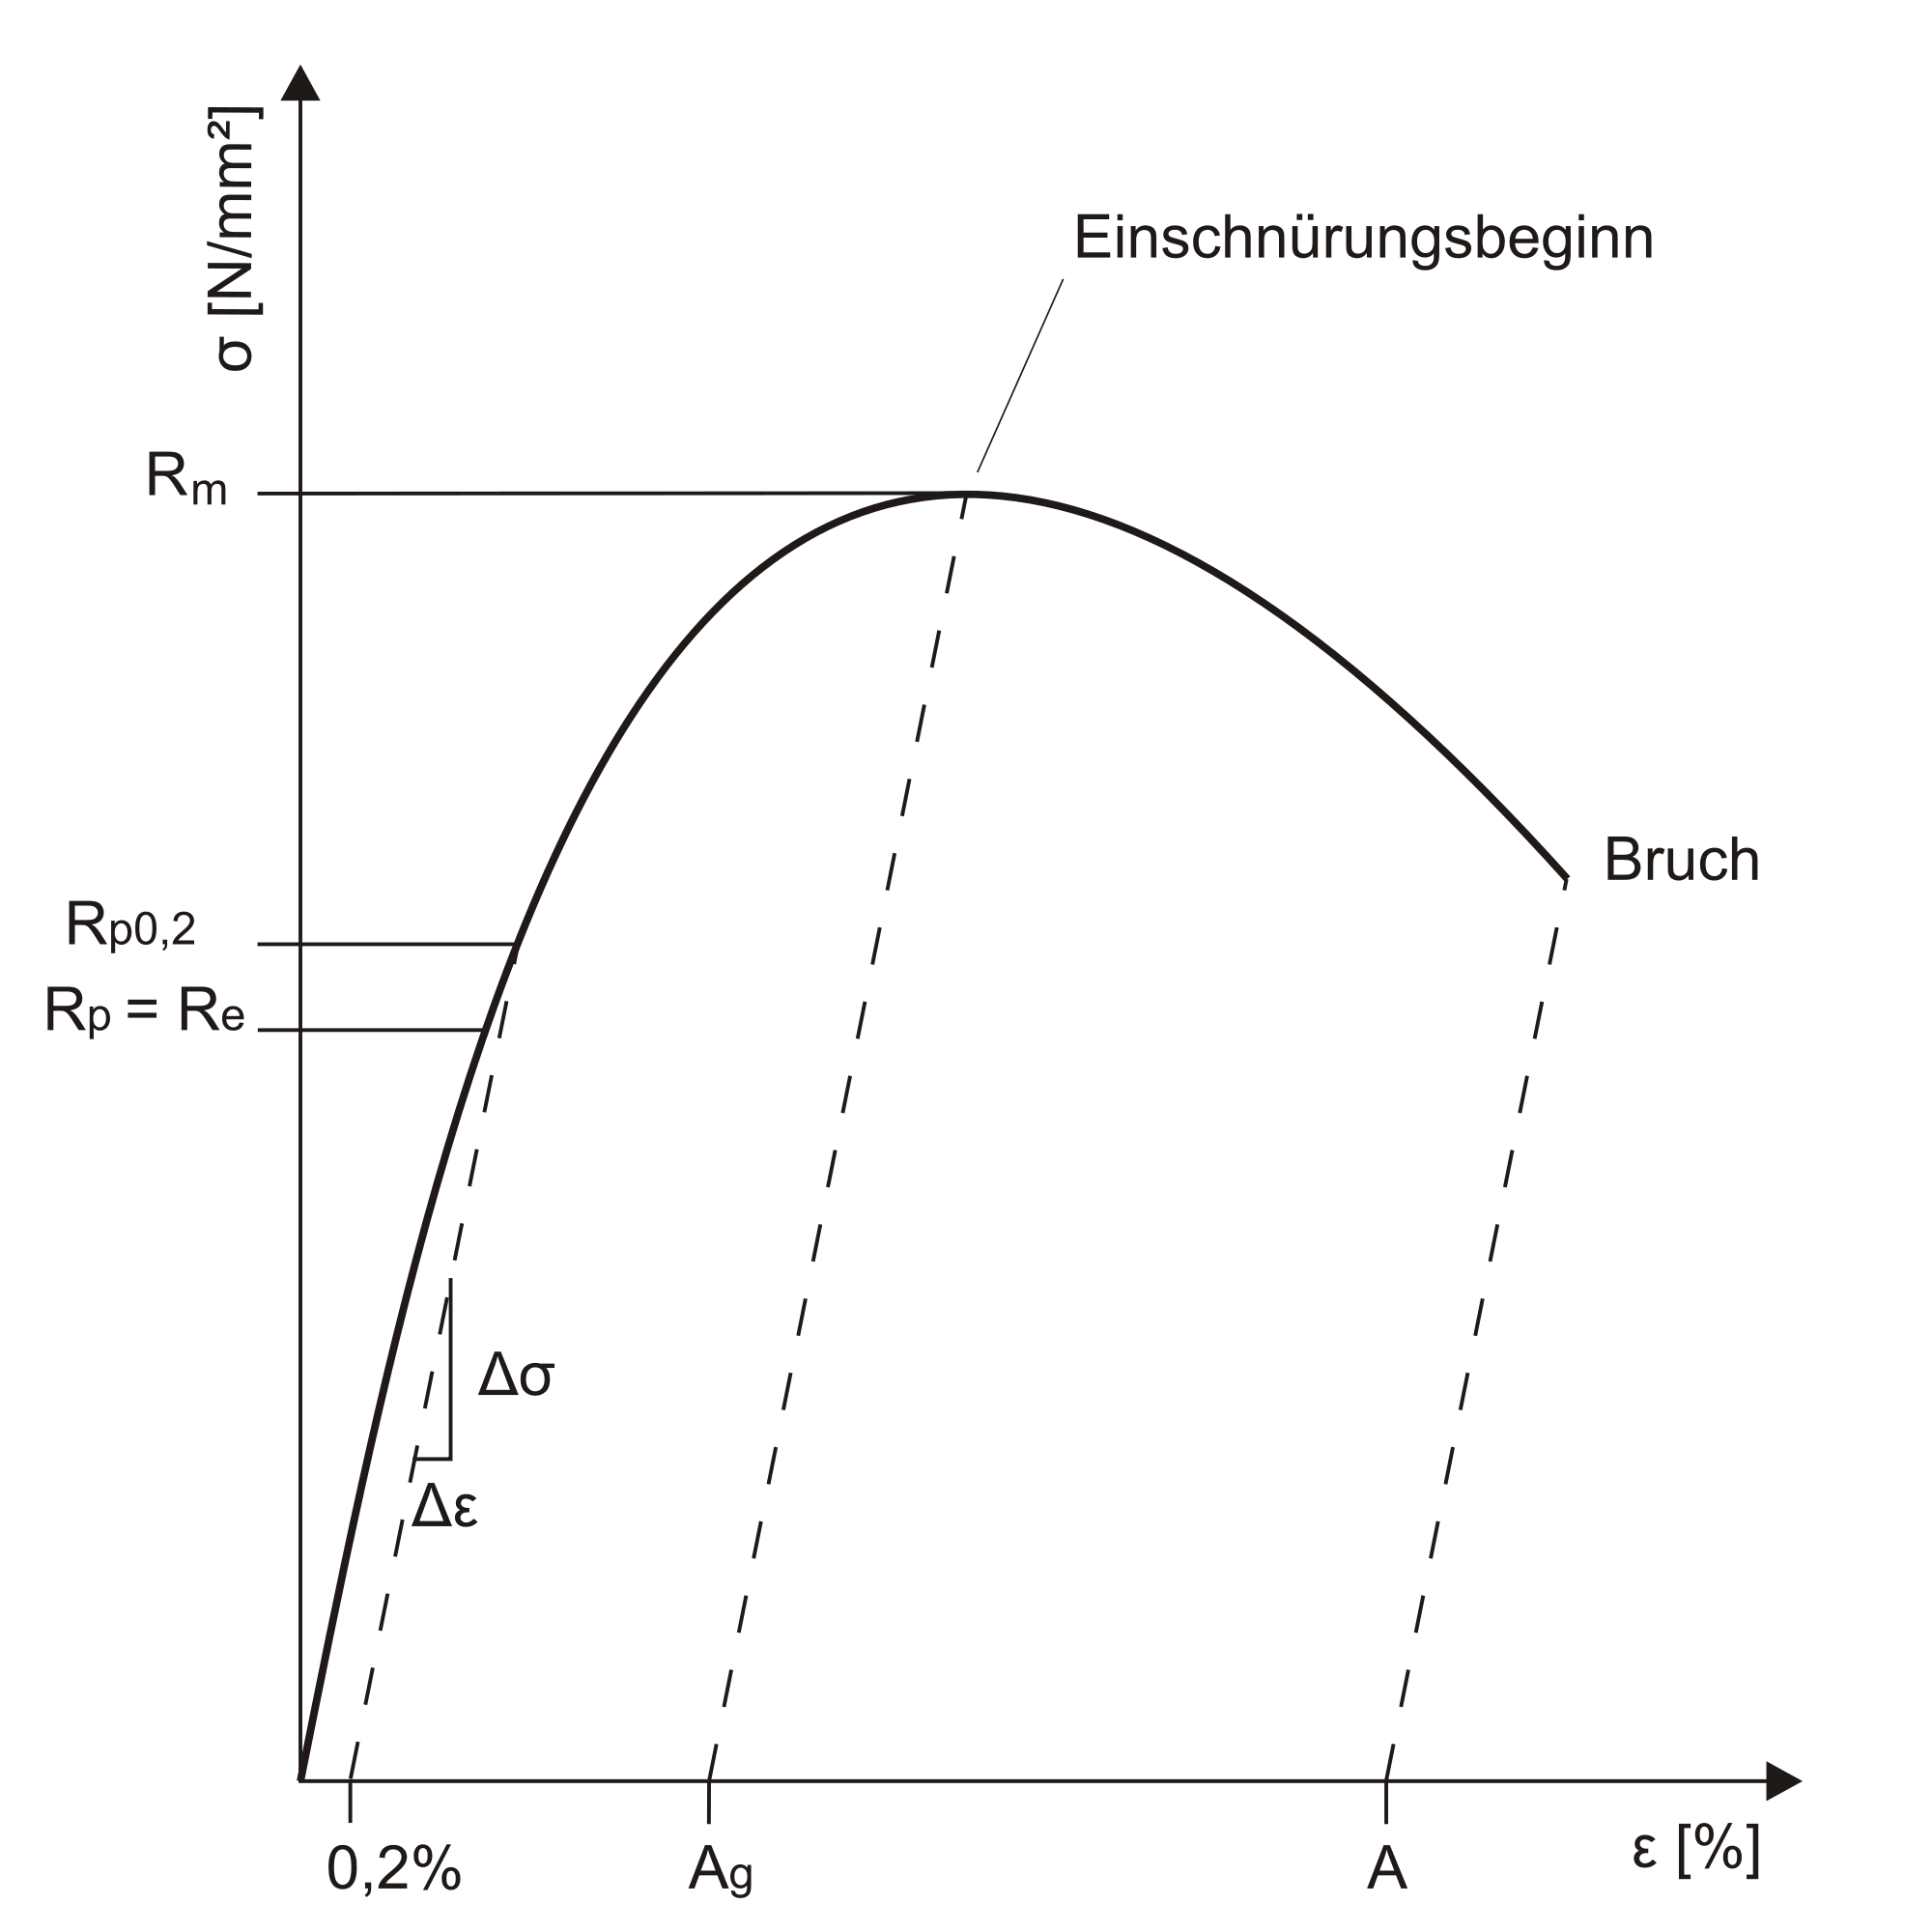
\includegraphics[height=0.5\textwidth]{medien/Spgs-Dehnungs-Kurve_Dehngrenze.png}
	\\
	\tiny{Quelle:https://de.wikipedia.org/wiki/Spannungs-Dehnungs-Diagramm}
\end{frame}
